\documentclass{standalone}
\usepackage{tikz}
\usetikzlibrary {arrows.meta}
\pagestyle{empty}

\begin{document}
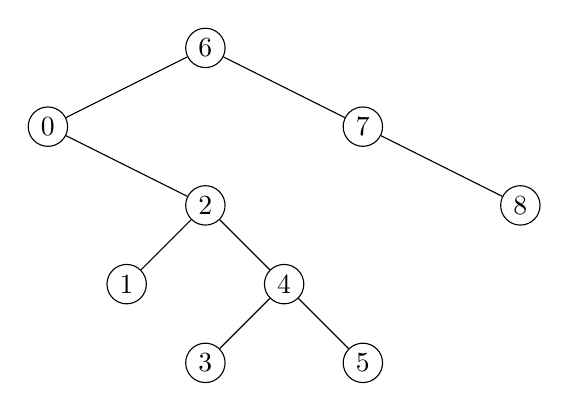
\begin{tikzpicture}

\tikzstyle{every node}=[draw,shape=circle,minimum size=0.5cm,inner sep=0pt,anchor=center];

% Draw the splay tree nodes
\node (n6) at (2,4) {6};
\node (n0) at (0,3) {0};
\node (n7) at (4,3) {7};
\node (n2) at (2,2) {2};
\node (n8) at (6,2) {8};
\node (n1) at (1,1) {1};
\node (n4) at (3,1) {4};
\node (n3) at (2,0) {3};
\node (n5) at (4,0) {5};

% Links between the nodes
\draw (n6) -- (n0)
(n6) -- (n7)
(n0) -- (n2)
(n7) -- (n8)
(n2) -- (n1)
(n2) -- (n4)
(n4) -- (n3)
(n4) -- (n5);


\tikzset{every edge/.append style = {-Stealth,dashed,gray}};

% Visitation: normal edition
%\path[every node/.style={font=\sffamily\small}]
%  (n6) edge[bend right,orange] node [right] {} (n0)
%  (n0) edge[bend right,orange] node [right] {} (n2)
%  (n2) edge[bend right,orange] node [right] {} (n1)
%  (n1) edge[bend right,teal] node [right] {} (n2)
%  (n2) edge[bend right,orange] node [right] {} (n4)
%  (n4) edge[bend right,orange] node [right] {} (n3)
%  (n3) edge[bend right,teal] node [right] {} (n4)
%  (n4) edge[bend right,orange] node [right] {} (n5)
%%  (n5) edge[bend right,violet] node [right] {} (n4)
%%  (n4) edge[bend right,violet] node [right] {} (n2)
%%  (n2) edge[bend right,violet] node [right] {} (n0)
%  (n5) edge[violet] node [right] {} (n6)
%  (n0) edge[bend right,teal] node [right] {} (n6)
%  (n6) edge[bend right,orange] node [right] {} (n7)
%  (n7) edge[bend right,orange] node [right] {} (n8);
%  (n8) edge[bend right,violet] node [right] {} (n7)
%  (n7) edge[bend right,violet] node [right] {} (n6);


\end{tikzpicture}
\end{document}
